
\section{Numerical Results}\label{sec:numRes}
In the following figures, the simulations of the model for different distributions can be found.
\begin{figure}[h]
  \centering
  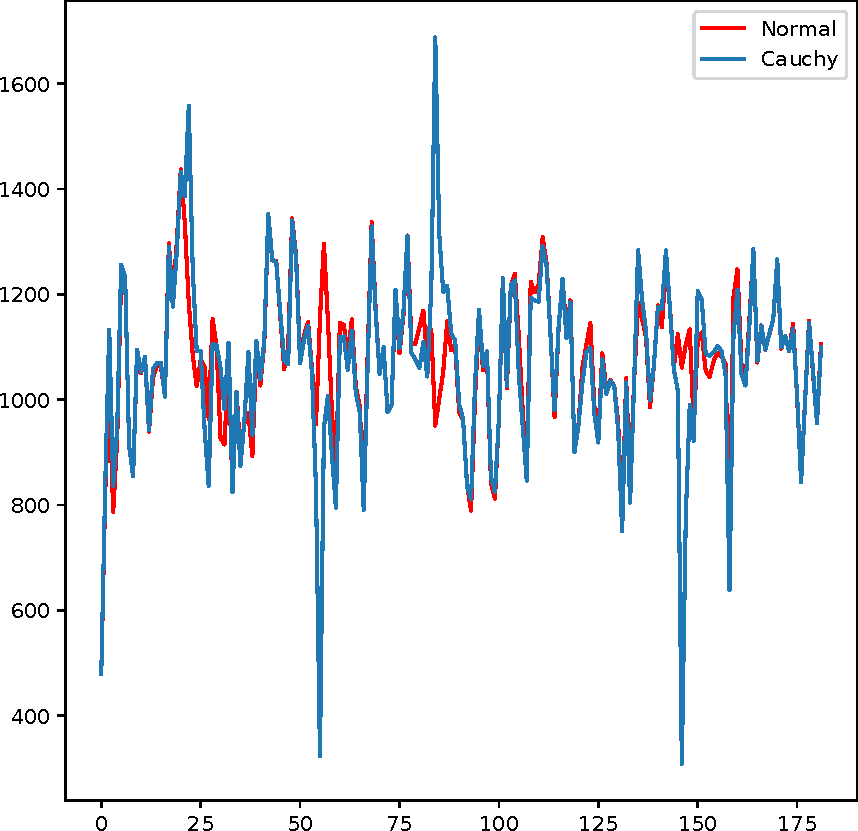
\includegraphics[scale=0.45]{files/sims.pdf}
  \caption{Results using Normal and Cauchy distribution.}
  \label{fig:cauchy}
\end{figure}

\begin{figure}[h]
  \centering
  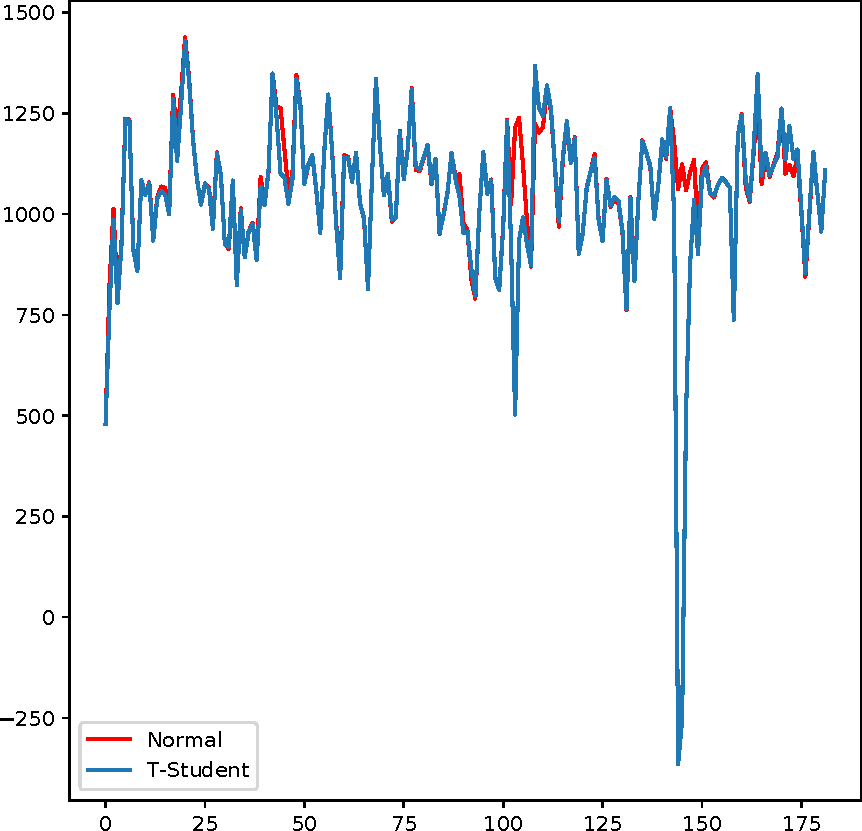
\includegraphics[scale=0.45]{files/simt.pdf}
  \caption{Results using Normal and T-Student distribution.}
  \label{fig:t}
\end{figure}

It is important to notice, that for Figs \ref{fig:cauchy}, \ref{fig:t}
the time series has unusual behavior as it has some random
spikes. This is due to the nature of the distributions used, as they
generate outliers.

On the other hand, it is seen that for every
simulation the normal distribution and the other one have a similar
pattern for most of the time simulated. In this manner, these
distributions do not change drastically the behavior of the time
series.

Furthermore, the simulations in this work gave a higher value that the
one presented in \cite{li2014armax}. This is an unexpected behavior
and raises the question of which simulation is correct. This could be
explained for this work, as it was not know the noise values that the
original paper used.
